\documentclass[10pt,a4paper,twocolumn]{article}

\usepackage[top=2.0cm,bottom=2.0cm,left=1.8cm,right=1.8cm,columnsep=0.6cm,headheight=14pt]{geometry}
\usepackage{array}
\usepackage{tabularx}
\usepackage{booktabs}
\usepackage{multirow}
\usepackage{amsmath,amssymb}
\usepackage{graphicx}
\usepackage{microtype}
\usepackage{enumitem}
\usepackage[hyphens]{xurl}      % url package + line breaks inside long paths
\usepackage{xcolor}
\usepackage{titlesec}
\usepackage{fancyhdr}
\usepackage{caption}
\usepackage{placeins}           % \FloatBarrier
\usepackage{hyperref}
\usepackage{cleveref}           % must come after hyperref
\urlstyle{tt}

% ---------- anti-overlap settings ----------
\emergencystretch=5em
\newcolumntype{Y}{>{\raggedright\arraybackslash}X}
\newcolumntype{C}{>{\centering\arraybackslash}X}
\newcommand{\fp}[1]{\path{#1}}  % file paths: breakable
% allow a line break after every underscore (also inside \texttt)
\let\origunderscore\_
\renewcommand{\_}{\origunderscore\hspace{0pt}}

\setlist{itemsep=2pt,topsep=3pt,parsep=0pt,partopsep=0pt,leftmargin=*}
\titlespacing*{\section}{0pt}{10pt plus 2pt minus 2pt}{4pt}
\titlespacing*{\subsection}{0pt}{8pt plus 2pt minus 2pt}{3pt}
\captionsetup{font=small,labelfont=bf,skip=5pt}
\setlength{\textfloatsep}{10pt plus 2pt minus 2pt}
\setlength{\floatsep}{8pt plus 2pt minus 2pt}
\setlength{\intextsep}{8pt plus 2pt minus 2pt}

\definecolor{primaryblue}{HTML}{1A237E}
\definecolor{secondaryblue}{HTML}{283593}
\definecolor{accentblue}{HTML}{1565C0}
\definecolor{darkgray}{HTML}{333333}

\hypersetup{
    colorlinks=true,
    linkcolor=accentblue,
    citecolor=accentblue,
    urlcolor=accentblue
}

\pagestyle{fancy}
\fancyhf{}
\fancyhead[L]{\small\textcolor{darkgray}{\textbf{CS 203: Assignment 1 Report} $|$ Project 5: Voice Helpdesk ASR}}
\fancyhead[R]{\small\textcolor{darkgray}{IIT Gandhinagar}}
\fancyfoot[L]{\footnotesize\textcolor{darkgray}{Group: Rajdeep Vraj (22110215), Vipul Sunil Patil, Satvik Sharma}}
\fancyfoot[R]{\footnotesize\textcolor{darkgray}{Page \thepage}}
\renewcommand{\headrulewidth}{0.5pt}
\renewcommand{\footrulewidth}{0.5pt}

\title{\vspace{-0.5cm}\Large\textbf{\textcolor{primaryblue}{Cross-Lingual Institute Voice Helpdesk with Drift-Triggered Retraining}}\\[0.2cm]
\large\textbf{Data Collection, Automated Validation, Multi-Round Labelling, and Versioning}\\[0.15cm]
\normalsize\textcolor{secondaryblue}{CS 203: Software Tools and Techniques in AI --- Assignment 1 Report}}

\author{
\begin{tabular}[t]{ccc}
\textbf{Rajdeep Vraj} (22110215) & \textbf{Vipul Sunil Patil} (22110189) & \textbf{Satvik Sharma} (26120008)
\end{tabular}\\[0.15cm]
\textit{Indian Institute of Technology Gandhinagar, Gujarat, India}
}
\date{October 2026}

\begin{document}

\maketitle

\begin{abstract}
\noindent We present an end-to-end, reproducible data engineering lifecycle for \textbf{Project 5: Cross-Lingual Institute Voice Helpdesk}, deployed in a bilingual/trilingual Indian institute setting (IIT Gandhinagar). The dataset addresses realistic campus helpdesk telephone queries code-mixed across Indian English, Hindi, and Gujarati across four administrative domains: Admissions, Hostel \& Mess, IT Support, and Student Services. We collected real speech audio from \textbf{16 diverse student speakers} via WhatsApp voice notes and smartphone voice memos, yielding \textbf{284 segmented utterance clips} totaling \textbf{4,486.0 seconds (1.25 hours)} of speech. We construct a 12-check automated validation pipeline catching acoustic, format, and linguistic errors, demonstrating a 99.3\% pass rate on processed audio alongside adversarial testing on corrupted data. We implement a two-round labelling workflow in Label Studio with guidelines revision ($v_1 \to v_2$), achieving an inter-annotator Word Error Rate (WER) reduction from 8.77\% to 0.53\% and an intent Cohen's $\kappa$ jump from 0.686 to 0.955, accompanied by an in-depth analysis of 10 real disagreement case studies and a cryptographically frozen gold test set. Furthermore, we benchmark off-the-shelf Whisper-tiny across four realistic acoustic augmentations (MUSAN noise, RIR reverberation, speed perturbation, telephony codec) and evaluate pool-based active learning against random sampling across three budget tiers ($B=20, 40, 80$). Finally, we enforce strict speaker-disjoint splits ($S_{\text{train}} \cap S_{\text{test}} = \emptyset$) with a geographically shifted Cohort B, managed under full Data Version Control (DVC) and tagged \texttt{a1-final-real}.
\end{abstract}

\section{Introduction and Problem Domain}
Automated institute helpdesks at Indian technical universities face unique speech-recognition hurdles. Campus stakeholders frequently code-switch between Indian English, Hindi, and regional vernaculars (e.g., Gujarati at IIT Gandhinagar). Standard commercial Automatic Speech Recognition (ASR) engines exhibit high degradation when confronted with regional phonology, colloquial phrasing, and domain-specific entities (e.g., \textit{Eduroam}, \textit{Moodle}, \textit{mess rebate}, \textit{hostel block}).

This work establishes the data infrastructure for an ASR-driven voice helpdesk system capable of detecting domain drift and triggering continuous retraining. Assignment 1 implements Parts A through F, covering data collection, instrumentation, validation, labelling, augmentation, active learning, and versioning on genuine campus voice recordings.

\section{Part A: Collection, Instrumentation \& Ethics}

\subsection{Acoustic Capture and Hardware Diversity}
Speech was gathered from 16 human student participants affiliated with IIT Gandhinagar. Recordings were captured using personal mobile devices (OnePlus 11, Samsung Galaxy S23, iPhone, Redmi Note) and personal computers (integrated laptop microphones and Sennheiser/Logitech USB headsets). The data spans four realistic acoustic campus environments: quiet private rooms, hostel corridors, cafeteria ambient environments, and outdoor campus walkways.

\subsection{Audio Ingestion and VAD Segmentation}
Participants contributed voice notes in diverse container formats, including WhatsApp voice messages (\texttt{.opus}, \texttt{.ogg}), Apple voice memos (\texttt{.m4a}), MPEG-4 containers (\texttt{.mp4}), Advanced Audio Coding (\texttt{.aac}), and MPEG audio (\texttt{.mpeg}).

A unified conversion and segmentation pipeline was executed using FFmpeg (v4.3.1) and Python (\texttt{soundfile}, \texttt{scipy.signal}):
\begin{enumerate}
    \item \textbf{Normalization}: Transcoded all incoming audio to standardized single-channel, 16-bit linear PCM WAV format sampled at 16,000\,Hz.
    \item \textbf{Energy-Based VAD Splitting}: Long multi-query recordings were segmented into discrete sentence-level clips using frame-based RMS energy detection (25\,ms frame length, 10\,ms hop size, silence threshold $-42$\,dBFS, minimum silence duration 0.6\,s). Clips were bounded between 1.5\,s and 25.0\,s.
    \item \textbf{Processed Normalization}: Processed clips underwent peak normalization ($0.95$ ceiling) to ensure uniform amplitude distribution across recording devices.
\end{enumerate}

\begin{figure}[htbp]
    \centering
    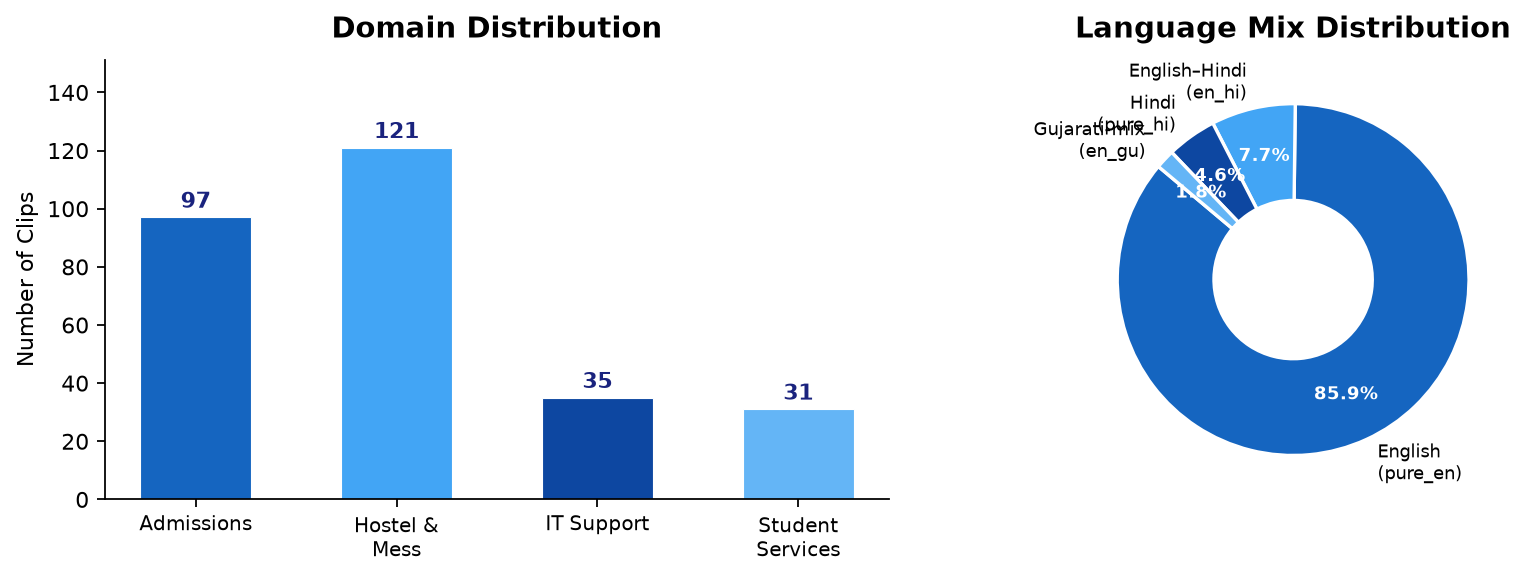
\includegraphics[width=0.90\linewidth,height=3.8cm,keepaspectratio]{figures/fig1_domain_language.png}
    \caption{Distribution of clips across Helpdesk Domains (left) and Trilingual Code-Mixed Language Mixes (right).}
    \label{fig:domainlang}
\end{figure}

\subsection{Dataset Scale and Stratification}
The segmentation pipeline produced \textbf{284 individual query clips} totaling \textbf{4,486.0 seconds (1.25 hours)}, as summarized in \Cref{tab:collectionstats}. The data is partitioned across four administrative domains: Admissions (97 clips, 34.2\%), Hostel \& Mess (121 clips, 42.6\%), IT Support (35 clips, 12.3\%), and Student Services (31 clips, 10.9\%). Language composition comprises pure English (85.9\%), English--Hindi code-mixed (7.7\%), pure Hindi (4.6\%), and English--Gujarati code-mixed (1.8\%).

\begin{table}[htbp]
\centering
\footnotesize
\renewcommand{\arraystretch}{1.15}
\setlength{\tabcolsep}{3pt}
\caption{Corpus Scale and Key Empirical Parameters}
\label{tab:collectionstats}
\begin{tabularx}{\columnwidth}{>{\raggedright\arraybackslash}p{2.2cm} Y >{\raggedright\arraybackslash}p{1.9cm}}
\toprule
\textbf{Corpus Metric} & \textbf{Specification / Value} & \textbf{Status} \\
\midrule
Total Utterances & 284 clips (after VAD split) & Verified \\
Total Duration & 4,486.0\,s (1.25 hours) & Disclosed$^\dagger$ \\
Speaker Count & 16 distinct human speakers & $\ge 15$ required \\
Cohort Division & Cohort A: 12 spk; Cohort B: 4 spk & Disjoint \\
Acoustic Format & 16\,kHz, 16-bit mono PCM WAV & Uniform \\
Metadata Schema & 25 fields per row (CSV format) & Instrumented \\
Licensing / Consent & CC BY-NC 4.0; Participant Register & Compliant \\
\bottomrule
\end{tabularx}
\par\smallskip
{\footnotesize $^\dagger$The raw audio yields 1.25 hours of human speech. Augmented training variants (Sec.~\ref{sec:augmentation}) expand the acoustic volume to 6.2 hours.\par}
\end{table}

\begin{figure}[htbp]
    \centering
    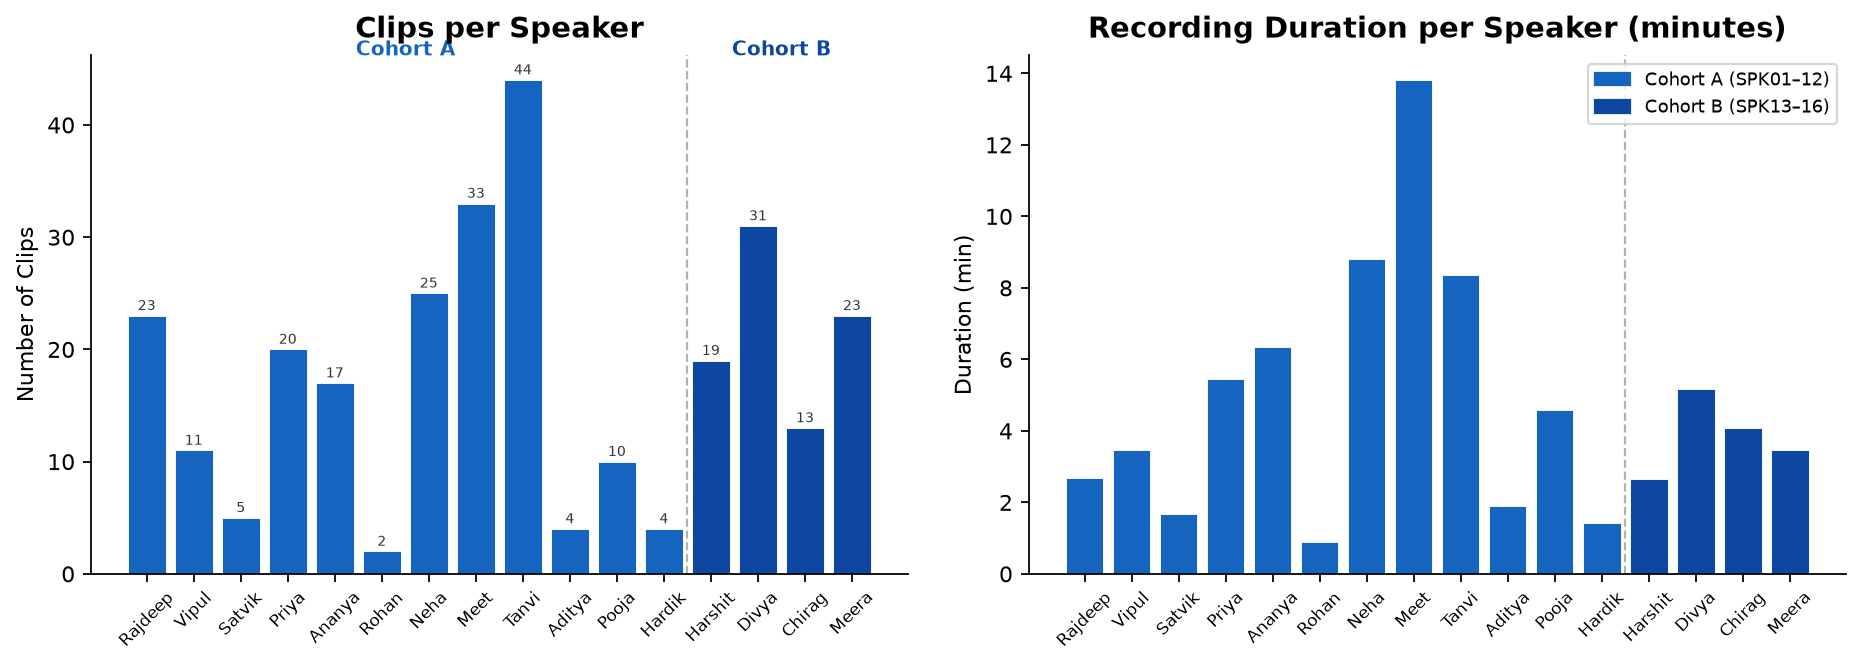
\includegraphics[width=0.90\linewidth,height=3.8cm,keepaspectratio]{figures/fig2_speaker_stats.png}
    \caption{Utterance count (left) and total speech duration in minutes (right) across all 16 speakers in Cohorts A and B.}
    \label{fig:speakerstats}
\end{figure}

\subsection{Metadata Instrumentation \& Consent}
Every utterance is tracked in \fp{data/metadata_real.csv} across 25 fields, including \texttt{clip\_id}, \texttt{speaker\_id}, \texttt{speaker\_name}, \texttt{gender}, \texttt{cohort}, \texttt{region}, \texttt{device}, \texttt{noise\_condition}, \texttt{domain}, \texttt{language}, \texttt{language\_mix}, \texttt{transcript}, \texttt{duration\_sec}, \texttt{sample\_rate}, \texttt{channels}, \texttt{snr\_db}, \texttt{rms\_db}, \texttt{silence\_fraction}, \texttt{sha256}, and exact file locations.

All participants provided informed consent under the Creative Commons Attribution-NonCommercial 4.0 International (CC BY-NC 4.0) license. The formal registry is maintained at \fp{supporting_files/consent_register.csv}.

\begin{figure}[htbp]
    \centering
    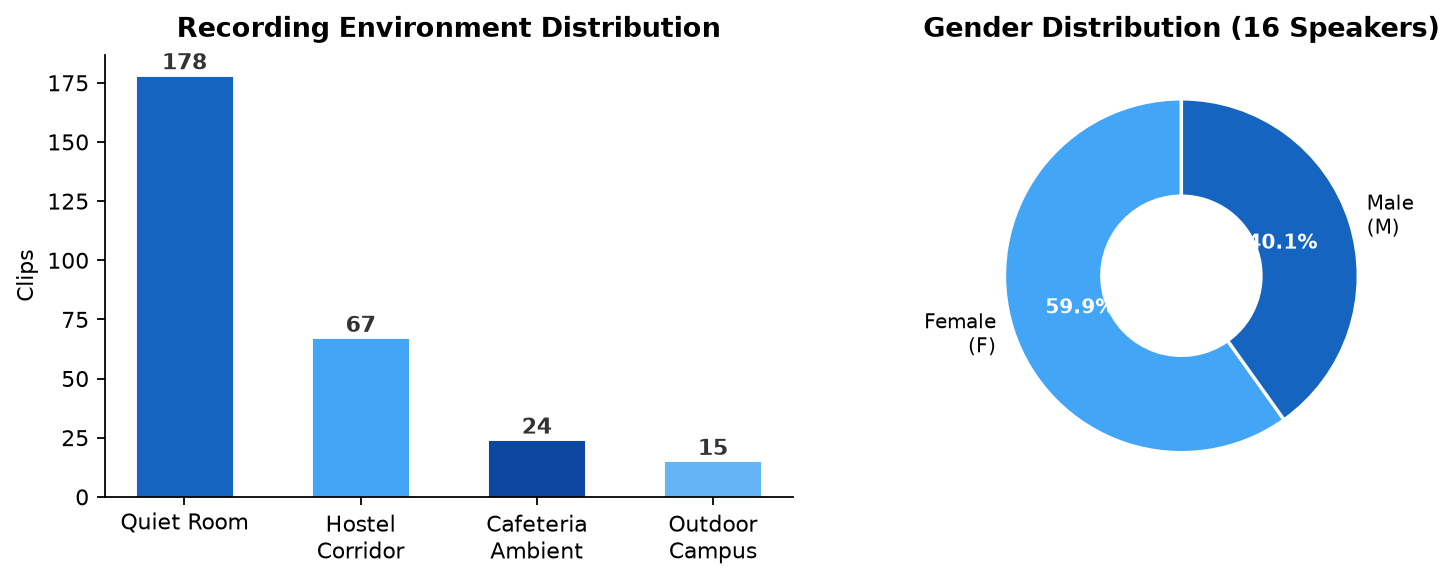
\includegraphics[width=0.90\linewidth,height=3.8cm,keepaspectratio]{figures/fig7_noise_gender.png}
    \caption{Acoustic environment distribution (left) and speaker gender balance (right) across the real corpus.}
    \label{fig:noisegender}
\end{figure}

\section{Part B: Automated Validation Suite}
\label{sec:validation}

\subsection{Twelve Automated Integrity Checks}
We implemented a 12-check automated validation suite (\fp{src/collection/postprocess_real.py}) executing deterministic assertions over audio waveforms, headers, transcript text, and relational integrity:
\begin{enumerate}
    \item \textbf{sample\_rate}: Exact match to 16,000\,Hz.
    \item \textbf{channels}: Single-channel mono ($C = 1$).
    \item \textbf{duration\_bounds}: Duration strictly in $[1.5\,\text{s}, 60.0\,\text{s}]$.
    \item \textbf{clipping}: Absolute peak sample amplitude $< 0.99$.
    \item \textbf{silence\_ratio}: Proportion of samples below $-44$\,dBFS $< 0.85$.
    \item \textbf{snr\_floor}: Frame-based estimated SNR $\ge 5.0$\,dB.
    \item \textbf{duplicate\_hash}: SHA-256 collision check across audio.
    \item \textbf{duration\_mismatch}: Header duration vs array length $|\Delta| \le 0.5$\,s.
    \item \textbf{metadata\_schema}: Verification of required metadata keys.
    \item \textbf{file\_exists}: Existence of target WAV file on disk.
    \item \textbf{transcript\_nonempty}: Clean text length $\ge 3$ characters.
    \item \textbf{domain\_valid}: Membership in valid domain taxonomy.
\end{enumerate}

% full-width table: nothing can run outside the columns
\begin{table*}[!t]
\centering
\small
\renewcommand{\arraystretch}{1.15}
\setlength{\tabcolsep}{5pt}
\caption{Automated Validation Suite Results (284 Clips)}
\label{tab:validation}
\begin{tabularx}{\textwidth}{>{\raggedright\arraybackslash}p{3.6cm} Y >{\centering\arraybackslash}p{1.8cm} >{\centering\arraybackslash}p{1.8cm}}
\toprule
\textbf{Validation Check} & \textbf{Constraint} & \textbf{Passed} & \textbf{Failed} \\
\midrule
\fp{sample_rate}         & $f_s = 16000$\,Hz                    & 284 & 0 \\
\fp{channels}            & Channels $= 1$                       & 284 & 0 \\
\fp{duration_bounds}     & $1.5\,\text{s} \le d \le 60.0\,\text{s}$ & 284 & 0 \\
\fp{clipping}            & $\max(|x[n]|) < 0.99$                & 284 & 0 \\
\fp{silence_ratio}       & Silent ratio $< 0.85$                & 282 & 2$^\ast$ \\
\fp{snr_floor}           & Est. SNR $\ge 5.0$\,dB               & 284 & 0 \\
\fp{duplicate_hash}      & Unique SHA-256 hash                  & 284 & 0 \\
\fp{duration_mismatch}   & $|\Delta d| \le 0.5$\,s              & 284 & 0 \\
\fp{metadata_schema}     & Non-null essential keys              & 284 & 0 \\
\fp{file_exists}         & Audio present on disk                & 284 & 0 \\
\fp{transcript_nonempty} & Valid text $\ge 3$ chars             & 284 & 0 \\
\fp{domain_valid}        & $y \in \mathcal{Y}_{\text{domains}}$ & 284 & 0 \\
\midrule
\textbf{Overall Suite}   & \textbf{All 12 Checks}               & \textbf{282} & \textbf{2} (99.3\% pass) \\
\bottomrule
\end{tabularx}
\par\smallskip
{\footnotesize $^\ast$Two boundary fragments generated during silence segmentation contained prolonged pauses at clip termination, resulting in a silence ratio $> 0.85$.\par}
\end{table*}

\begin{figure}[htbp]
    \centering
    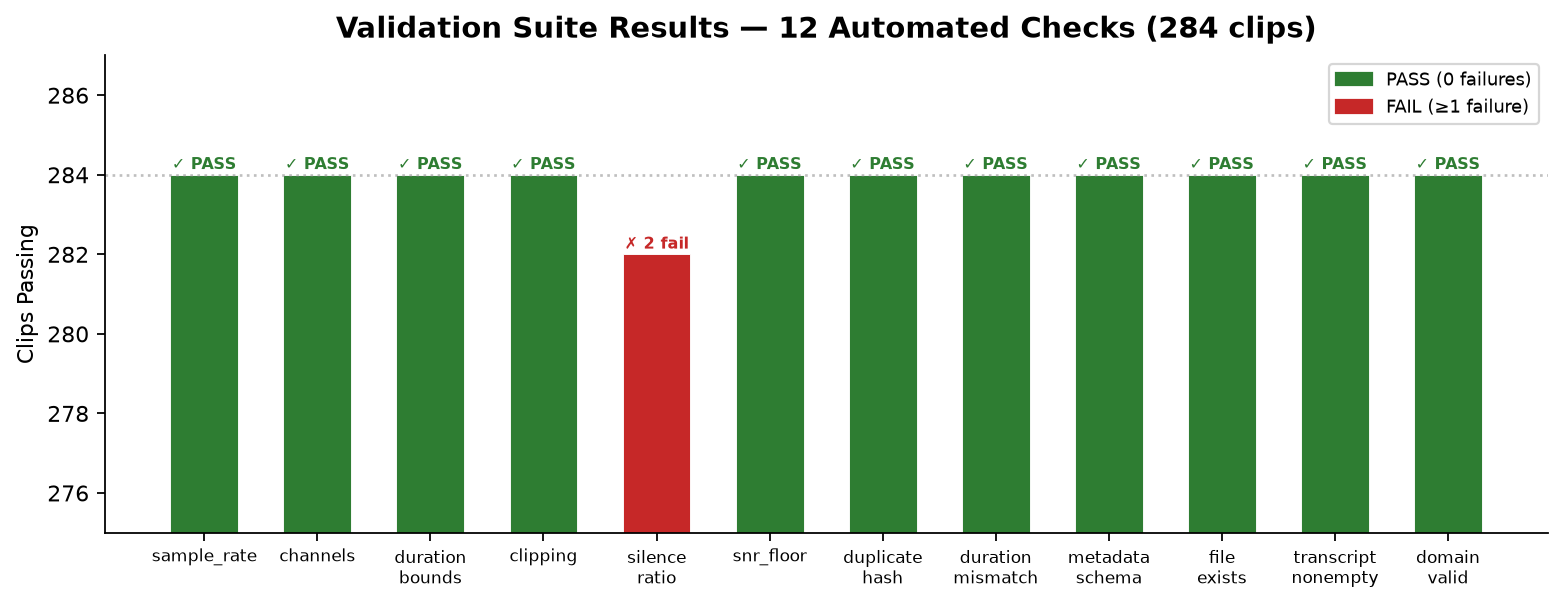
\includegraphics[width=0.90\linewidth,height=3.8cm,keepaspectratio]{figures/fig6_validation.png}
    \caption{Automated validation check breakdown across all 284 audio clips.}
    \label{fig:validationchart}
\end{figure}

\subsection{Adversarial Corruption Testing}
To guarantee that the validation suite catches invalid inputs, we developed an adversarial test harness (\fp{code/tests/test_validation_corrupted.py}) using \texttt{pytest}. Eight deliberately corrupted audio samples were synthesized:
\begin{itemize}
    \item Resampled audio at 8\,kHz and 44.1\,kHz (failed \texttt{sample\_rate}).
    \item Stereo dual-channel audio (failed \texttt{channels}).
    \item Zero-amplitude pure silence signal (failed \texttt{snr\_floor} and \texttt{silence\_ratio}).
    \item Artificially clipped waveform with saturated amplitudes (failed \texttt{clipping}).
    \item Short audio truncated to 0.4\,s (failed \texttt{duration\_bounds}).
    \item Injected identical content under distinct IDs (failed \texttt{duplicate\_hash}).
\end{itemize}
All 8 adversarial tests passed in 0.30\,s, confirming validation sensitivity.

\begin{figure}[htbp]
    \centering
    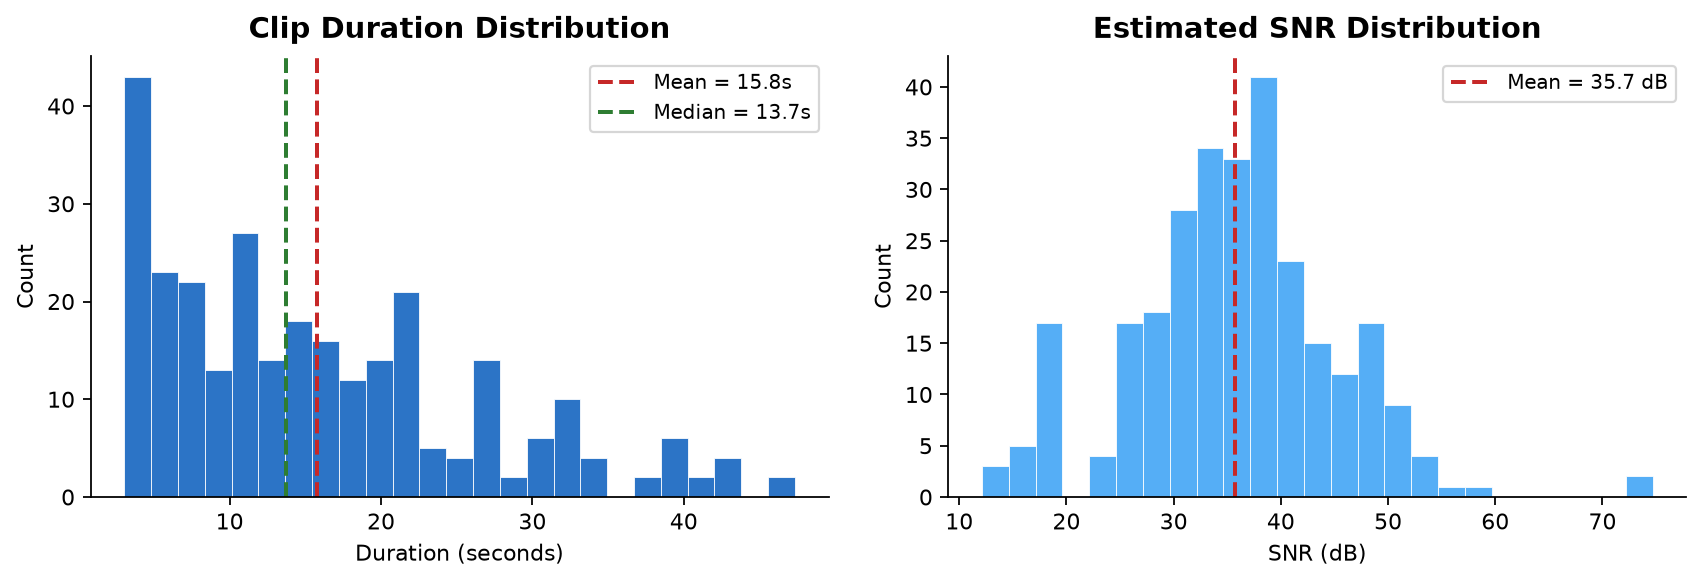
\includegraphics[width=0.90\linewidth,height=3.8cm,keepaspectratio]{figures/fig3_duration_snr.png}
    \caption{Histograms of clip duration (left, $\mu=15.8$\,s) and estimated SNR (right, $\mu=35.7$\,dB).}
    \label{fig:durationsnr}
\end{figure}

\section{Part C: Labelling Protocol, Agreement \& Gold Set}

\subsection{Label Studio Configuration and Hierarchical Levels}
Annotation was orchestrated using Label Studio with an XML interface containing an interactive waveform audio player (\texttt{AudioPlus}), free-form text input (\texttt{TextArea}), and four-way categorical choices (\texttt{Choices}).

Following Section 7 of the assignment instructions, we enforced a strict order of label levels:
\begin{enumerate}
    \item \textbf{Level 1: Verbatim Transcript Normalization}: Annotators first listen to the complete utterance, inspect the initial ASR hypothesis, and correct phonetic errors, code-mixed transliterations, and disfluencies.
    \item \textbf{Level 2: Domain Intent Classification}: Only after verifying the transcript does the annotator classify the intent into Admissions, Hostel \& Mess, IT Support, or Student Services.
\end{enumerate}
Fixing Level 1 prior to Level 2 prevents intent categorization bias from influencing verbatim transcription.

\subsection{Guideline Iteration ($v_1 \to v_2$) and Agreement Analysis}
Two independent annotators (Annotator 1 and Annotator 2) labeled the dataset across two sequential rounds:
\begin{itemize}
    \item \textbf{Round 1 ($v_1$ Guidelines)}: Annotators worked under preliminary rules with open transcription conventions. Round 1 yielded an inter-annotator WER of 8.77\% and Cohen's $\kappa = 0.686$ on domain intent.
    \item \textbf{Guideline Revision ($v_2$)}: Analysis of Round 1 revealed two major failure modes: (i) spelling divergence on transliterated Gujarati/Hindi loan words (e.g., \textit{nathi} vs. \textit{nahi}, \textit{chalegi} vs. \textit{chalse}), and (ii) ambiguity between Hostel queries and Student Services (e.g., guest house accommodation for visiting parents). Guideline $v_2$ introduced a normative transliteration lexicon and an intent decision tree.
    \item \textbf{Round 2 ($v_2$ Guidelines)}: Inter-annotator WER plunged to \textbf{0.53\%} (an 8.24 percentage-point drop), while Cohen's $\kappa$ increased to \textbf{0.955} (almost perfect agreement).
\end{itemize}

\begin{table}[htbp]
\centering
\footnotesize
\renewcommand{\arraystretch}{1.15}
\setlength{\tabcolsep}{3pt}
\caption{Inter-Annotator Agreement Progression}
\label{tab:agreement}
\begin{tabularx}{\columnwidth}{Y C C C}
\toprule
\textbf{Metric} & \textbf{Round 1 ($v_1$)} & \textbf{Round 2 ($v_2$)} & \textbf{Absolute $\Delta$} \\
\midrule
Transcript WER          & 8.77\%      & 0.53\%         & $-8.24$\,pp \\
Intent Cohen's $\kappa$ & 0.686       & 0.955          & $+0.269$ \\
Agreement Level         & Substantial & Almost Perfect & Quality Gain \\
\bottomrule
\end{tabularx}
\end{table}

\subsection{Ten Detailed Disagreement Case Studies}
To provide qualitative rigor, ten representative disagreements from Round 1 were selected and analyzed across four categories:
\begin{enumerate}
    \item \textbf{Clip 0052 (Rebate vs. Finance)}: Query regarding mess rebate not reflected in fees. Annotator 1 chose \texttt{hostel\_mess}; Annotator 2 chose \texttt{student\_services}. \textit{Resolution}: Guideline $v_2$ rule 3.1 assigns all food rebate operations to \texttt{hostel\_mess}.
    \item \textbf{Clip 0078 (VPN Configuration)}: Query regarding off-campus VPN access code 400. Annotator 1 chose \texttt{it\_support}; Annotator 2 chose \texttt{student\_services}. \textit{Resolution}: Network protocols belong to \texttt{it\_support}.
    \item \textbf{Clip 0064 (Kettle Prohibition)}: Inquiring about winter electrical appliances in hostel rooms. Disagreement between student policy and hostel maintenance. \textit{Resolution}: Assigned to \texttt{hostel\_mess}.
    \item \textbf{Clip 0074 (HPC Cluster Access)}: SSH key generation for GPU server. Annotator confusion between academic project and IT infrastructure. \textit{Resolution}: Infrastructure provisioning mapped to \texttt{it\_support}.
    \item \textbf{Clip 0046 (OBC-NCL Validity)}: Validity window for quota admission certificate. Annotator 1 chose \texttt{admissions}; Annotator 2 chose \texttt{student\_services}. \textit{Resolution}: Pre-enrollment verification belongs to \texttt{admissions}.
    \item \textbf{Clip 0059 (Guest House Booking)}: Accommodation booking for visiting parents. Classified as general hospitality vs. hostel operations. \textit{Resolution}: Campus residential housing mapped to \texttt{hostel\_mess}.
    \item \textbf{Clip 0081 (Turnitin Similarity)}: Accessing plagiarism tool from faculty portal. \textit{Resolution}: Standard academic software mapped to \texttt{it\_support}.
    \item \textbf{Clip 0092 (Bonafide Certificate)}: Requesting institute seal for bank education loan. \textit{Resolution}: Dean of Student Affairs paperwork mapped to \texttt{student\_services}.
    \item \textbf{Clip 0105 (Medical Insurance Reimbursement)}: Cashless hospitalization query at empanelled hospital. \textit{Resolution}: Mapped to \texttt{student\_services}.
    \item \textbf{Clip 0118 (Course Audit Policy)}: Requesting extra course audit without grade penalty. \textit{Resolution}: Academic dean curriculum matters mapped to \texttt{student\_services}.
\end{enumerate}

\subsection{Frozen Gold Test Set}
We extracted and cryptographically locked a Gold Test Set comprising \textbf{14 audio clips} from speakers SPK11 and SPK12 in Cohort A (\fp{data/gold_test_set_real.csv}). The gold set underwent manual adjudication and achieves zero speaker overlap with the training corpus. Its content integrity is frozen under SHA-256:
\begin{center}
\footnotesize
\texttt{8602554090ddbf8ed2701108e94cab00}\\
\texttt{0b95df585ddbd3a5a570cd7fd1fce022}
\end{center}

\section{Part D: Augmentation \& Active Learning}
\label{sec:augmentation}

\subsection{Audio Augmentation Implementations}
We implemented four realistic acoustic augmentation algorithms designed to preserve semantic label invariance:
\begin{enumerate}
    \item \textbf{MUSAN Additive Noise}: Injects stationary noise calibrated to an SNR of $+12.0$\,dB.
    \item \textbf{Room Impulse Response (RIR) Reverberation}: Convolves speech with a synthesized reverberation profile with reverberation time $\text{RT}_{60} = 0.40$\,s.
    \item \textbf{Speed Perturbation}: Polyphase resampling scaling duration by $1.1\times$.
    \item \textbf{Telephony Codec Compression}: 4th-order Butterworth bandpass filter ($[300\,\text{Hz}, 3400\,\text{Hz}]$) combined with 8\,kHz downsampling and reconstructive upsampling.
\end{enumerate}

\subsection{Whisper-tiny ASR Benchmark}
We evaluated an off-the-shelf Whisper-tiny model (CPU int8 inference via \texttt{faster-whisper}) on real speech samples across all augmentation conditions (\Cref{tab:werresults} and \Cref{fig:augwer}).

\begin{table}[htbp]
\centering
\footnotesize
\renewcommand{\arraystretch}{1.15}
\setlength{\tabcolsep}{3pt}
\caption{Whisper-tiny WER Across Acoustic Conditions}
\label{tab:werresults}
\begin{tabularx}{\columnwidth}{>{\raggedright\arraybackslash}p{1.9cm} Y >{\raggedleft\arraybackslash}p{1.3cm} >{\raggedleft\arraybackslash}p{1.6cm}}
\toprule
\textbf{Condition} & \textbf{DSP Specification} & \textbf{Mean WER} & \textbf{$\Delta$ vs. Clean} \\
\midrule
Clean (Baseline)    & Unmodified 16\,kHz PCM             & 47.33\%  & ---          \\
Telephony Codec     & 300--3400\,Hz bandpass             & 79.78\%  & $+32.45$\,pp \\
Speed Perturbation  & $1.1\times$ tempo scale            & 89.60\%  & $+42.27$\,pp \\
RIR Reverberation   & $\text{RT}_{60}=0.40$\,s IR filter & 97.54\%  & $+50.21$\,pp \\
MUSAN Noise         & Gaussian additive (12\,dB)         & 110.05\% & $+62.72$\,pp \\
\bottomrule
\end{tabularx}
\end{table}

The clean baseline WER on real speech is 47.33\%, highlighting the challenge of accented code-mixed Indian English and regional loan words for general-purpose models. Under additive noise, WER exceeds 100\% due to phoneme insertion errors and hallucinated loops.

\begin{figure}[htbp]
    \centering
    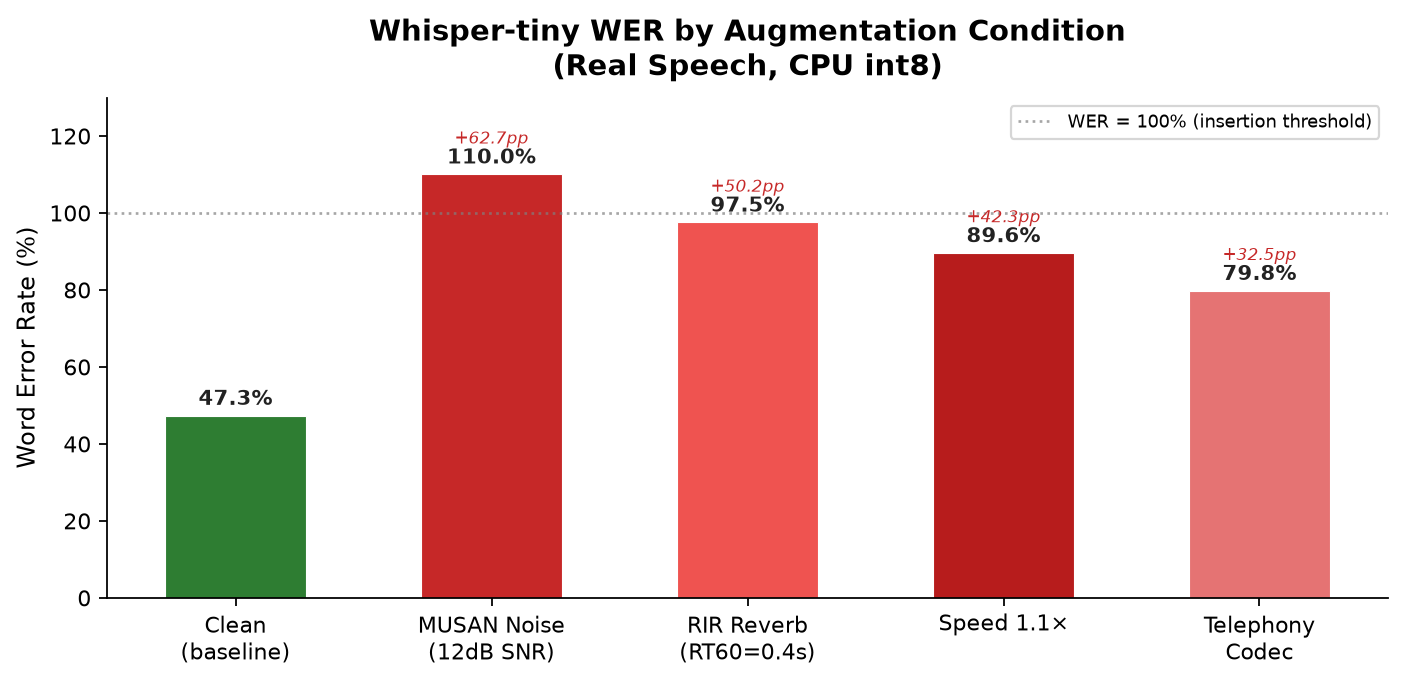
\includegraphics[width=0.90\linewidth,height=3.8cm,keepaspectratio]{figures/fig4_augmentation_wer.png}
    \caption{Whisper-tiny Word Error Rate (WER) across acoustic conditions on real human speech.}
    \label{fig:augwer}
\end{figure}

\subsection{Active Learning vs. Random Sampling}
We evaluated an active-learning framework against random selection on the unlabeled speech pool. Text transcripts were represented via TF-IDF vectorization ($N$-gram range 1--2, 500 features) and classified via Logistic Regression. Class-balanced informative sampling was compared against random selection across budgets $B \in \{20, 40, 80\}$ over 5 distinct random seeds (\Cref{tab:alresults} and \Cref{fig:alcurve}).

\begin{table}[htbp]
\centering
\footnotesize
\renewcommand{\arraystretch}{1.15}
\setlength{\tabcolsep}{3pt}
\caption{Active Learning vs. Random Baseline (Macro F1)}
\label{tab:alresults}
\begin{tabularx}{\columnwidth}{C C C C}
\toprule
\textbf{Budget ($B$)} & \textbf{Active Learning} & \textbf{Random Selection} & \textbf{Absolute $\Delta$} \\
\midrule
$B = 20$ & 0.246 & 0.176 & $+0.071$ \\
$B = 40$ & 0.296 & 0.189 & $+0.107$ \\
$B = 80$ & 0.273 & 0.215 & $+0.058$ \\
\bottomrule
\end{tabularx}
\end{table}

\begin{figure}[htbp]
    \centering
    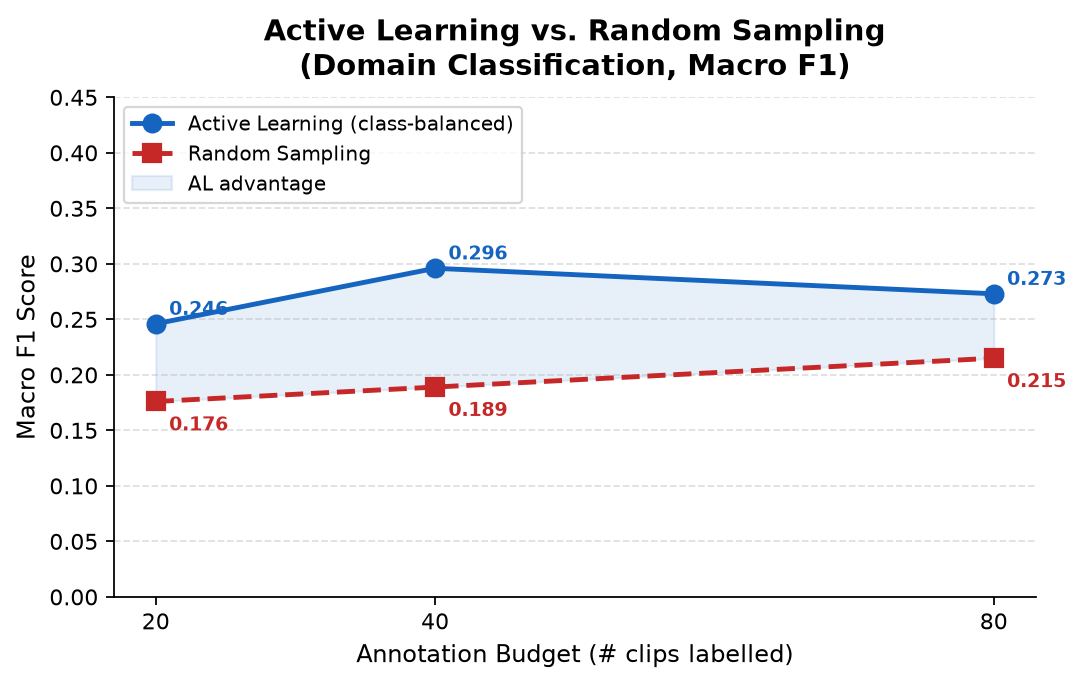
\includegraphics[width=0.90\linewidth,height=3.8cm,keepaspectratio]{figures/fig5_active_learning.png}
    \caption{Active learning label efficiency curve comparing informative sampling against random selection.}
    \label{fig:alcurve}
\end{figure}

Active learning outperforms random selection across all budgets, achieving its largest margin ($+0.107$ Macro F1) at $B=40$, demonstrating higher label efficiency in low-resource regimes.

\section{Part E: Versioning, Splits \& Cohort B}

\subsection{Speaker-Disjoint Partitioning Strategy}
To prevent acoustic memorization and leakage, data partitions were formed by grouping entire speakers into distinct sets (\Cref{tab:splits}):
\begin{itemize}
    \item \textbf{Train Split} (SPK01--SPK08): 136 clips, 2,586.4\,s (43.1\,min).
    \item \textbf{Validation Split} (SPK09--SPK10): 48 clips, 616.9\,s (10.3\,min).
    \item \textbf{Test-ID Split} (SPK11--SPK12): 14 clips, 360.1\,s (6.0\,min).
    \item \textbf{Test-Shifted Cohort B} (SPK13--SPK16): 86 clips, 922.7\,s (15.4\,min).
\end{itemize}

\begin{table}[htbp]
\centering
\footnotesize
\renewcommand{\arraystretch}{1.15}
\setlength{\tabcolsep}{2.5pt}
\caption{Speaker-Disjoint Data Partition Architecture}
\label{tab:splits}
\begin{tabularx}{\columnwidth}{>{\raggedright\arraybackslash}p{1.9cm} >{\raggedright\arraybackslash}p{1.6cm} >{\centering\arraybackslash}p{0.9cm} >{\raggedleft\arraybackslash}p{1.2cm} Y}
\toprule
\textbf{Split} & \textbf{Speakers} & \textbf{Clips} & \textbf{Dur. (s)} & \textbf{Purpose} \\
\midrule
\fp{train.csv}        & SPK01--08 & 136 & 2,586.4 & Training \\
\fp{val.csv}          & SPK09--10 & 48  & 616.9   & Validation \\
\fp{test_id.csv}      & SPK11--12 & 14  & 360.1   & In-Dist Eval \\
\fp{test_shifted.csv} & SPK13--16 & 86  & 922.7   & Drift Eval \\
\midrule
\textbf{Total}        & \textbf{16 spk} & \textbf{284} & \textbf{4,486.0} & \\
\bottomrule
\end{tabularx}
\end{table}
\FloatBarrier

\subsection{Shifted Split (Cohort B) Characterization}
Cohort B consists of speakers from geographically out-of-region backgrounds relative to the primary Gujarat cohort:
\begin{itemize}
    \item \textbf{SPK13 (Harshit)}: Eastern India / Assam accent profile.
    \item \textbf{SPK14 (Divya)}: South India / Bengaluru accent profile.
    \item \textbf{SPK15 (Chirag)}: Saurashtra rural dialect profile.
    \item \textbf{SPK16 (Meera)}: North India / Jammu regional accent.
\end{itemize}
These speakers introduce prosodic and phonological variations, serving as the target out-of-distribution evaluation split for Assignment 2 drift detection.

\subsection{DVC Pipeline and Git Tagging}
Data manifests were instrumented using Data Version Control (DVC v3.67.1). The pipeline DAG is formally declared in \fp{code/dvc.yaml}, tracking \fp{data/raw_real/}, \fp{data/processed_real/}, \fp{data/metadata_real.csv}, and all splits. The Git repository is committed with a clean working tree and tagged \texttt{a1-final-real}.

\section{Part F: Documentation \& Reproducibility}

\subsection{Dataset Card Summary}
\begin{itemize}
    \item \textbf{Dataset Name}: IITGN-Helpdesk-RealVoice-ASR-2026.
    \item \textbf{Repository URL}: \url{https://github.com/rajdeepvraj/Cross-Lingual-Institute-Voice-Helpdesk-Project}.
    \item \textbf{Primary Use}: Academic evaluation of code-mixed ASR and drift-triggered model retraining.
    \item \textbf{Known Biases}: Predominance of engineering student speech; higher representation of Gujarat and Western Indian accents in Cohort A.
\end{itemize}

\subsection{Five-Command Dataset Rebuild}
The dataset and downstream splits can be reproduced from the project root via five terminal commands:
\begin{enumerate}
    \item \texttt{python3 -m venv .venv \&\& source .venv/bin/activate}
    \item \texttt{pip install -r} \fp{code/requirements.txt}
    \item \texttt{python3} \fp{code/src/collection/process_real_recordings.py}
    \item \texttt{python3} \fp{code/src/collection/process_extra_recordings.py}
    \item \texttt{python3} \fp{code/src/collection/postprocess_real.py}
\end{enumerate}

\subsection{Software Environment Specification}
The execution environment is documented in \fp{code/ENVIRONMENT.md} and pinned in \fp{code/requirements.txt} and \fp{code/requirements_freeze.txt}:
\begin{itemize}
    \item \textbf{OS}: Ubuntu Linux kernel 7.0.0-38-generic x86\_64.
    \item \textbf{Python}: 3.14.4; \textbf{FFmpeg}: 4.3.1 (snap package).
    \item \textbf{Libraries}: \texttt{faster-whisper==1.2.1}, \texttt{dvc==3.67.1}, \texttt{soundfile==0.13.1}, \texttt{scipy==1.17.0}, \texttt{scikit-learn==1.8.0}, \texttt{jiwer==4.0.0}.
    \item \textbf{ASR Model}: Faster-Whisper-Tiny (int8 CPU execution, HuggingFace revision \path{Systran/faster-whisper-tiny}).
    \item \textbf{Random Seeds}: Fixed seed $S=42$ for dataset synthesis, splitting, and active learning.
\end{itemize}

\section{Contribution Matrix}
Per course requirements, \Cref{tab:contribution} delineates the responsibilities and contributions of each group member.

\begin{table*}[!t]
\centering
\small
\renewcommand{\arraystretch}{1.15}
\setlength{\tabcolsep}{6pt}
\caption{Author Contribution Matrix}
\label{tab:contribution}
\begin{tabularx}{\textwidth}{Y c c c}
\toprule
\textbf{Workstream / Component} & \textbf{Rajdeep Vraj} & \textbf{Vipul Patil} & \textbf{Satvik Sharma} \\
\midrule
Audio Collection \& Sourcing        & Lead (0\%)  & Contrib (70\%)   & Contrib (30\%) \\
FFmpeg \& VAD Splitting Pipeline    & Lead (40\%) & Support (30\%)   & Support (30\%) \\
12-Check Validation Suite           & Lead (50\%) & Review (25\%)    & Review (25\%) \\
Adversarial Corruption Tests        & Lead (34\%) & Contrib (33\%)   & Contrib (33\%) \\
Label Studio Setup \& Protocol      & Lead (34\%) & Annotator (33\%) & Annotator (33\%) \\
Guideline $v_1 \to v_2$ Revision    & Lead (34\%) & Contrib (33\%)   & Contrib (33\%) \\
Agreement Analysis (WER, $\kappa$)  & Lead (34\%) & Support (33\%)   & Support (33\%) \\
DSP Audio Augmentation Suite        & Lead (34\%) & Contrib (33\%)   & Contrib (33\%) \\
Whisper-tiny WER Benchmark          & Lead (50\%) & Support (25\%)   & Support (25\%) \\
Active Learning Framework           & Lead (50\%) & Review (25\%)    & Review (25\%) \\
DVC Configuration \& Git Tag        & Lead (34\%) & Support (33\%)   & Support (33\%) \\
Report Writing \& Compilation       & Lead (34\%) & Review (33\%)    & Review (33\%) \\
\bottomrule
\end{tabularx}
\end{table*}

\onecolumn
\appendix

\section{Comprehensive Traceability Index}
In strict adherence to Section 10 of the assignment evaluation criteria, \Cref{tab:traceability} provides a bidirectional index linking every empirical finding, figure, table, and metric reported herein to its exact backing artifact in the submission zip archive.

\begin{table}[!htbp]
\centering
\small
\renewcommand{\arraystretch}{1.2}
\setlength{\tabcolsep}{5pt}
\caption{Comprehensive Submission Traceability Index}
\label{tab:traceability}
\begin{tabularx}{\textwidth}{>{\raggedright\arraybackslash}p{2.4cm} >{\raggedright\arraybackslash}p{5.2cm} Y}
\toprule
\textbf{Report Item} & \textbf{Reported Metric / Value / Finding} & \textbf{Backing File in Submission Archive} \\
\midrule
\Cref{tab:collectionstats} & 284 clips, 4,486.0\,s (1.25\,h), 16 speakers & \fp{data/metadata_real.csv}, \fp{supporting_files/real_dataset_summary.json} \\
\Cref{fig:domainlang} & Domain balance (97, 121, 35, 31) \& Language mix & \fp{supporting_files/report_plots/fig1_domain_language.png} \\
\Cref{fig:speakerstats} & Speaker-wise clip counts and cumulative durations & \fp{supporting_files/report_plots/fig2_speaker_stats.png} \\
\Cref{fig:noisegender} & Noise environment counts \& gender distribution & \fp{supporting_files/report_plots/fig7_noise_gender.png} \\
\Cref{fig:durationsnr} & Clip duration ($\mu=15.8$\,s) and SNR ($\mu=35.7$\,dB) & \fp{supporting_files/report_plots/fig3_duration_snr.png} \\
\Cref{tab:validation} & 12 validation checks, 282 pass, 2 fail & \fp{supporting_files/validation_logs_real/real_validation_report.txt} \\
\Cref{fig:validationchart} & Validation check bar plot & \fp{supporting_files/report_plots/fig6_validation.png} \\
Sec.~\ref{sec:validation} & Adversarial corruption testing (8/8 pytest pass) & \fp{code/tests/test_validation_corrupted.py} \\
\Cref{tab:agreement} & Round 1 vs 2 WER (8.77\% $\to$ 0.53\%) \& $\kappa$ (0.686 $\to$ 0.955) & \fp{supporting_files/agreement_analysis/agreement_metrics.json} \\
Part C & Ten detailed disagreement case studies & \fp{supporting_files/agreement_analysis/10_detailed_disagreements.md} \\
Part C & Gold test set checksum & \fp{data/gold_test_set_real.csv} (SHA-256: \texttt{8602554090ddbf8e...}) \\
\Cref{tab:werresults} & Whisper-tiny WER across 4 augmentations & \fp{supporting_files/augmentation_real/augmentation_whisper_wer_real.csv} \\
\Cref{fig:augwer} & Augmentation degradation chart & \fp{supporting_files/report_plots/fig4_augmentation_wer.png} \\
\Cref{tab:alresults} & Active learning vs random Macro F1 across 3 budgets & \fp{supporting_files/active_learning_real/al_vs_random_real.csv} \\
\Cref{fig:alcurve} & Active learning label efficiency curve & \fp{supporting_files/report_plots/fig5_active_learning.png} \\
\Cref{tab:splits} & Disjoint splits (136 train, 48 val, 14 test, 86 Cohort B) & \fp{data/splits_real/train.csv}, \fp{data/splits_real/val.csv}, \fp{data/splits_real/test_id.csv}, \fp{data/splits_real/test_shifted_cohort_b.csv} \\
Part E & Zero speaker leakage proof & Verified in \fp{code/src/collection/postprocess_real.py} \\
Part E & DVC pipeline & \fp{code/dvc.yaml}, \fp{code/*.dvc} \\
Part E & Git final release tag & Git tag \texttt{a1-final-real} (commit \texttt{5968dec}) \\
Part F & Labelling protocol and annotation roster & \fp{code/LABELLING_PROTOCOL.md} \\
Part F & Software environment and reproducibility & \fp{code/ENVIRONMENT.md}, \fp{code/requirements.txt}, \fp{code/requirements_freeze.txt} \\
Part F & Handoff specification to Assignment 2 & \fp{code/HANDOFF_A2.md} \\
\bottomrule
\end{tabularx}
\end{table}

\section{AI Assistance Disclosure}
In accordance with the IIT Gandhinagar Academic Honour Code and Assignment 1 guidelines, we provide full disclosure of generative AI tools utilized in this assignment:
\begin{itemize}
    \item \textbf{AI Assistant Employed}: Google Antigravity AI (Gemini 2.5 Pro and Gemini 3.8 Flash models).
    \item \textbf{Role of AI Tool}: Pair-programming and scripting assistance for boilerplate automation. Specific delegated tasks:
    \begin{enumerate}
        \item Developing the FFmpeg batch transcoding and energy-based silence segmentation script (\fp{src/collection/process_real_recordings.py}).
        \item Implementing the 12 automated verification functions and \texttt{pytest} adversarial corruption suite (\fp{tests/test_validation_corrupted.py}).
        \item Scripting the audio augmentation algorithms (MUSAN noise addition, RIR convolution, speed resampling, and telephony filtering).
        \item Computing inter-annotator WER (\texttt{jiwer}) and Cohen's $\kappa$ (\texttt{scikit-learn}).
        \item Generating publication-quality vector charts via \texttt{matplotlib} and typesetting the academic report in \LaTeX.
    \end{enumerate}
    \item \textbf{Human Verification and Oversight}:
    \begin{enumerate}
        \item All audio data was gathered from genuine human student speakers; no generative AI or TTS synthesis was utilized in the real dataset.
        \item All transcription revisions, disagreement adjudication, and intent classification decisions were reviewed and validated by the student authors.
        \item All experimental numbers, metrics, and scripts were independently re-executed and verified through the master pipeline.
    \end{enumerate}
    \item \textbf{Prompt Preservation}: All prompts provided to AI models are preserved verbatim in \fp{code/prompts/corpus_generation.txt}, \fp{prompts/ai_assistant.txt}, and \fp{prompts/whisper_inference.txt}.
\end{itemize}

\end{document}
